%----------------------------------------%
%		       Prima slide	     	     %
%	Osservabili per reticolo 100 x 100   %
%----------------------------------------%
\begin{frame}
    \frametitle{Osservabili per reticolo $100 \times 100$}
    \framesubtitle{Ising 2D}

    \centering
    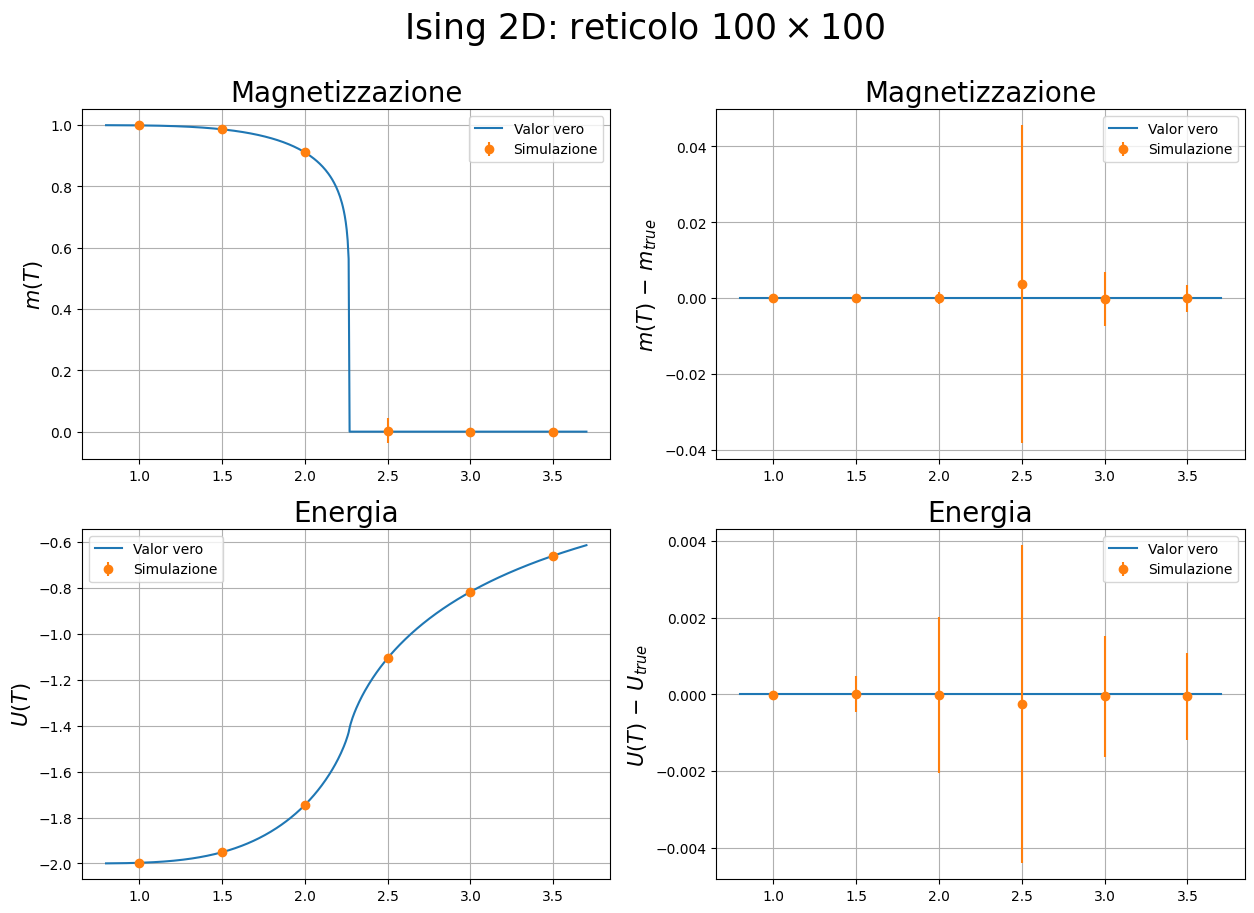
\includegraphics[width=0.65\textwidth]{Immagini/backupIsing2D/obs_100.png}

\end{frame}



%----------------------------------------%
%		      Seconda slide	     	     %
%	Osservabili per reticolo 100 x 100   %
%----------------------------------------%
\begin{frame}
    \frametitle{Osservabili per reticolo $200 \times 200$}
    \framesubtitle{Ising 2D}

    \centering
    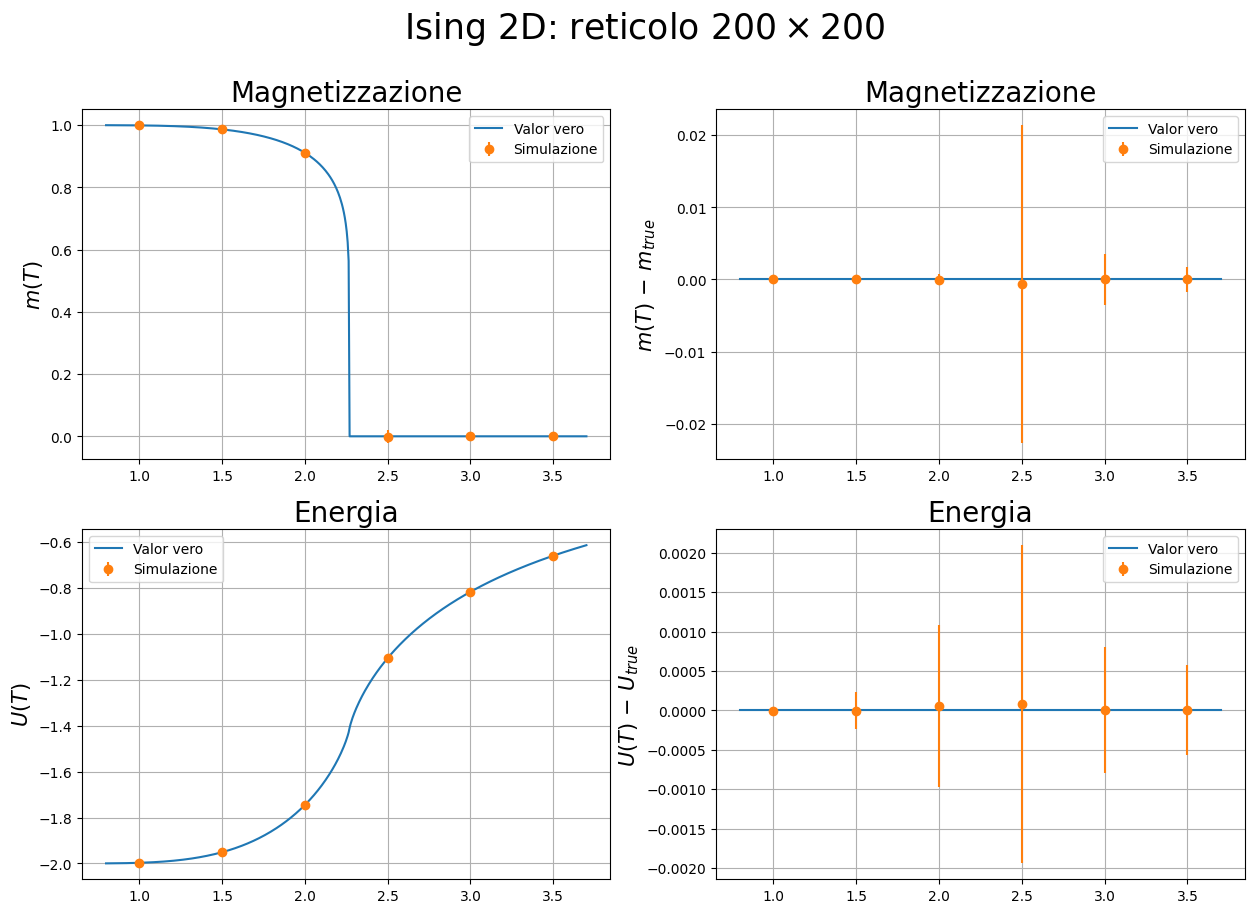
\includegraphics[width=0.65\textwidth]{Immagini/backupIsing2D/obs_200.png}

\end{frame}



%----------------------------------------%
%		       Terza slide	     	     %
%	Osservabili per reticolo 300 x 300   %
%----------------------------------------%
\begin{frame}
    \frametitle{Osservabili per reticolo $300 \times 300$}
    \framesubtitle{Ising 2D}

    \centering
    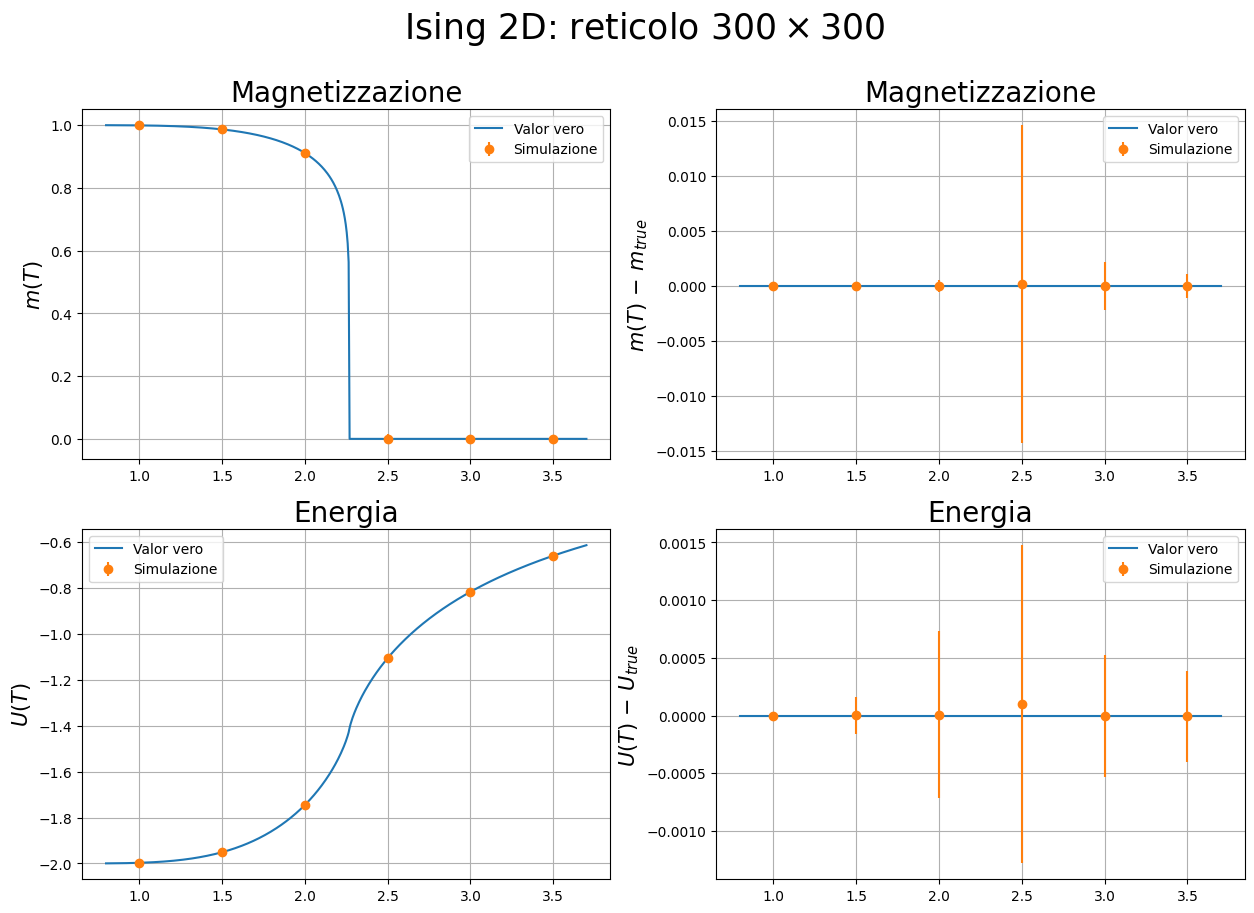
\includegraphics[width=0.65\textwidth]{Immagini/backupIsing2D/obs_300.png}

\end{frame}



%----------------------------------------%
%		       Quarta slide	     	     %
%	Osservabili per reticolo 400 x 400   %
%----------------------------------------%
\begin{frame}
    \frametitle{Osservabili per reticolo $400 \times 400$}
    \framesubtitle{Ising 2D}

    \centering
    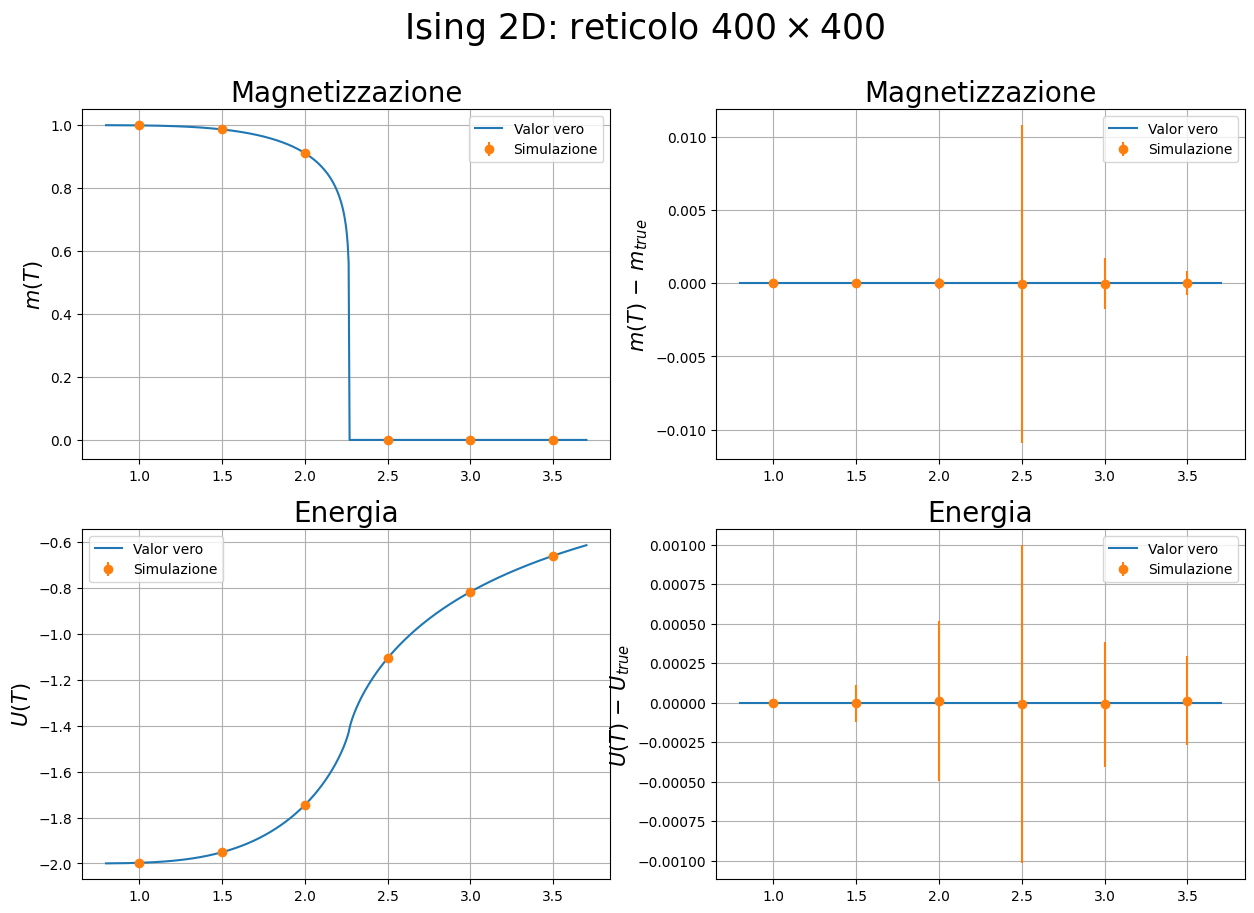
\includegraphics[width=0.65\textwidth]{Immagini/backupIsing2D/obs_400.png}

\end{frame}



%----------------------------------------%
%		       Quinta slide	     	     %
%	Osservabili per reticolo 500 x 500   %
%----------------------------------------%
\begin{frame}
    \frametitle{Osservabili per reticolo $500 \times 500$}
    \framesubtitle{Ising 2D}

    \centering
    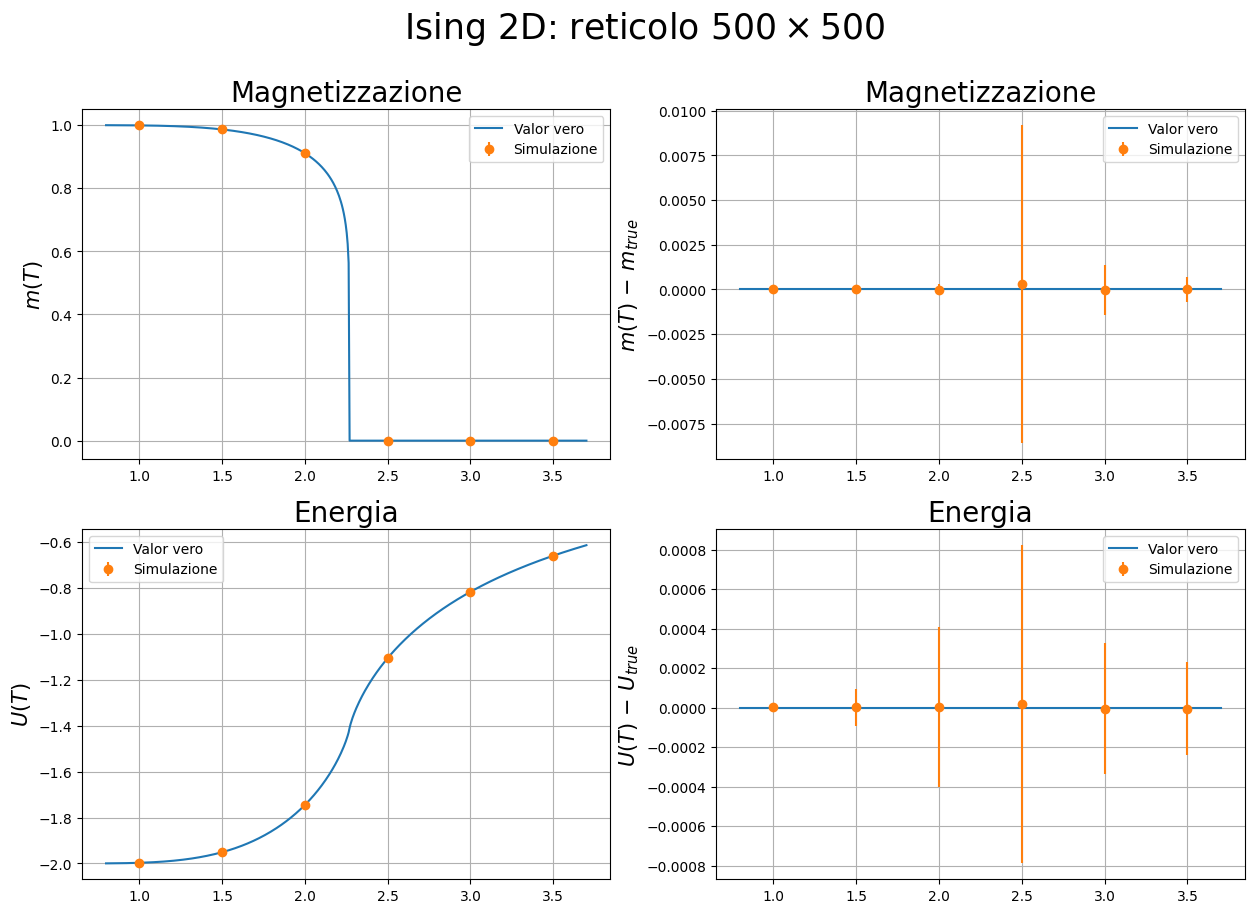
\includegraphics[width=0.65\textwidth]{Immagini/backupIsing2D/obs_500.png}

\end{frame}



%----------------------------------------%
%		        Sesta slide	     	     %
%	      Suscettività magnetica         %
%----------------------------------------%
\begin{frame}
    \frametitle{Suscettività}
    \framesubtitle{Ising 2D}

    \begin{columns}
        \begin{column}{0.6\textwidth}

            \centering
            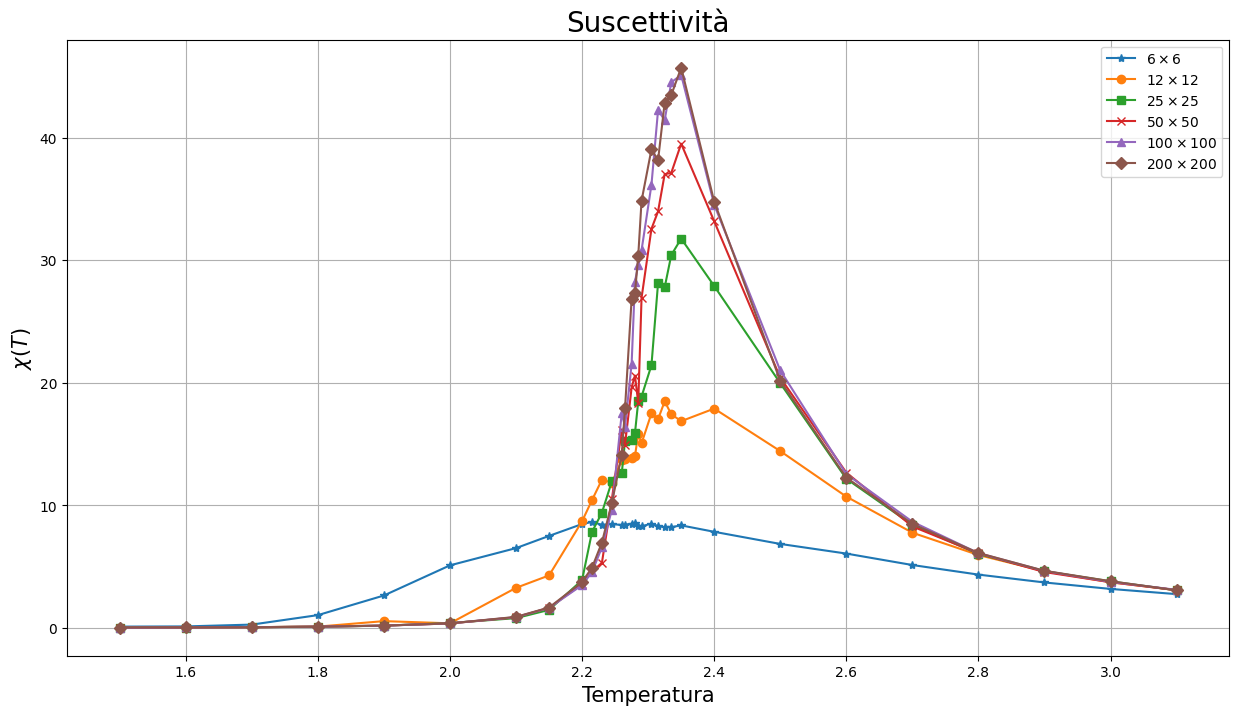
\includegraphics[width=\textwidth]{Immagini/backupIsing2D/chi.png}

        \end{column}
    
        \begin{column}{0.4\textwidth}

            \begin{itemize}[itemsep=0.5em, label=$\diamond$]
                \item Transizione di fase solo nel limite termodinamico
                \item Aumenta N, meglio risolto è il picco
                \item $N \to \infty$ implica $T_{max} \to T_c^+$
            \end{itemize}
            
        \end{column}
    \end{columns}

\end{frame}



%----------------------------------------%
%		      Settima slide	     	     %
%	      Suscettività magnetica         %
%----------------------------------------%
\begin{frame}
    \frametitle{Suscettività: Metropolis vs Wolff}
    \framesubtitle{Ising 2D}

    \begin{columns}
        \begin{column}{0.5\textwidth}

            \centering
            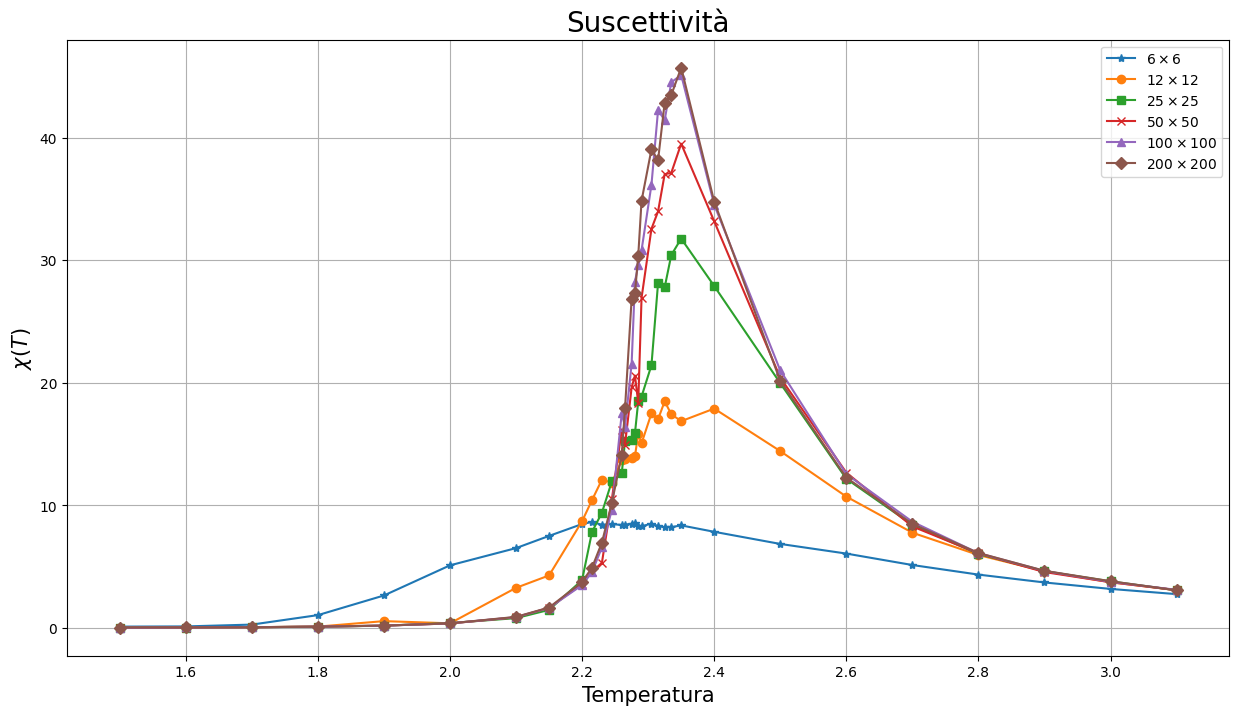
\includegraphics[width=\textwidth]{Immagini/backupIsing2D/chi.png}

        \end{column}
    
        \begin{column}{0.5\textwidth}

            \centering
            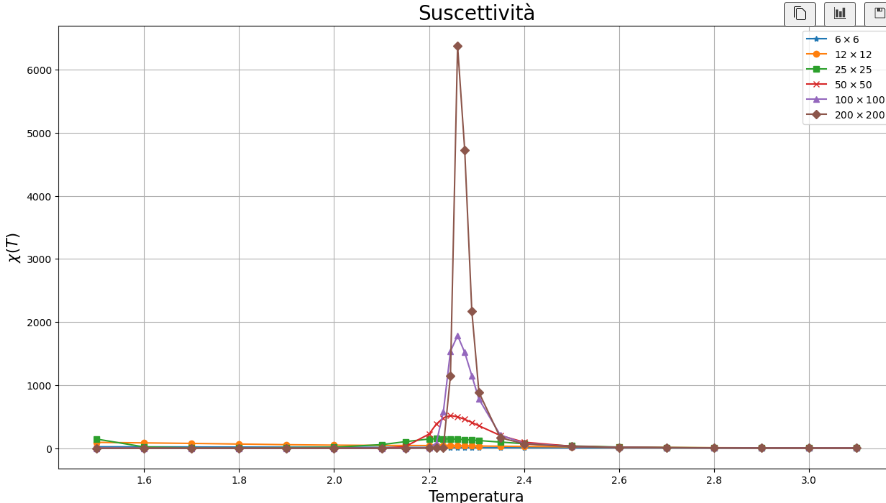
\includegraphics[width=\textwidth]{Immagini/backupIsing2D/chi_w.png}
            
        \end{column}
    \end{columns}

\end{frame}



%----------------------------------------%
%		      Ottava slide	     	     %
%	      Suscettività magnetica         %
%----------------------------------------%
\begin{frame}
    \frametitle{Suscettività: confronto Wolff}
    \framesubtitle{Ising 2D}

    \begin{columns}
        \begin{column}{0.5\textwidth}

            \centering
            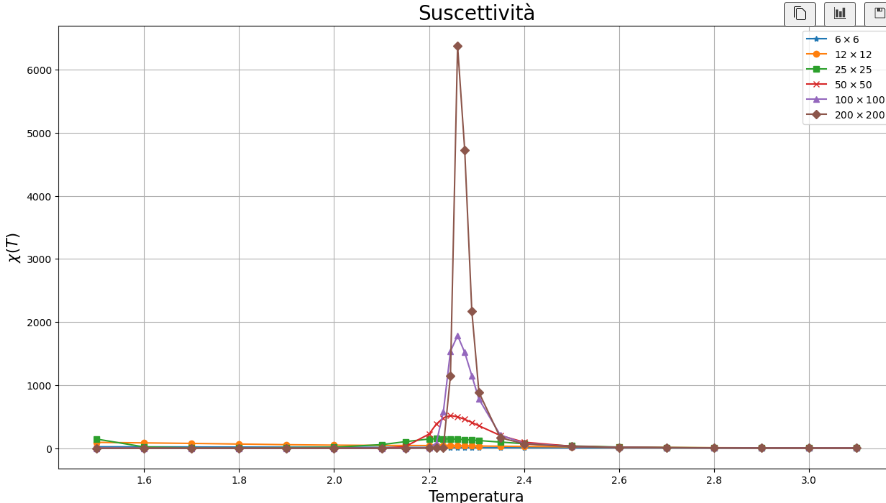
\includegraphics[width=\textwidth]{Immagini/backupIsing2D/chi_w.png}

        \end{column}
    
        \begin{column}{0.5\textwidth}

            \centering
            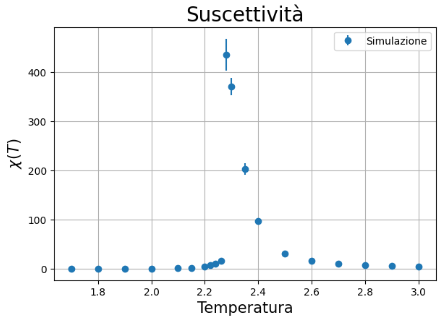
\includegraphics[width=\textwidth]{Immagini/backupIsing2D/chi_w1.png}
            
        \end{column}
    \end{columns}

\end{frame}